% PEaC Architecture Figure Description
% For inclusion in Elsevier CAS-SC template

\begin{figure}[ht]
    \centering
    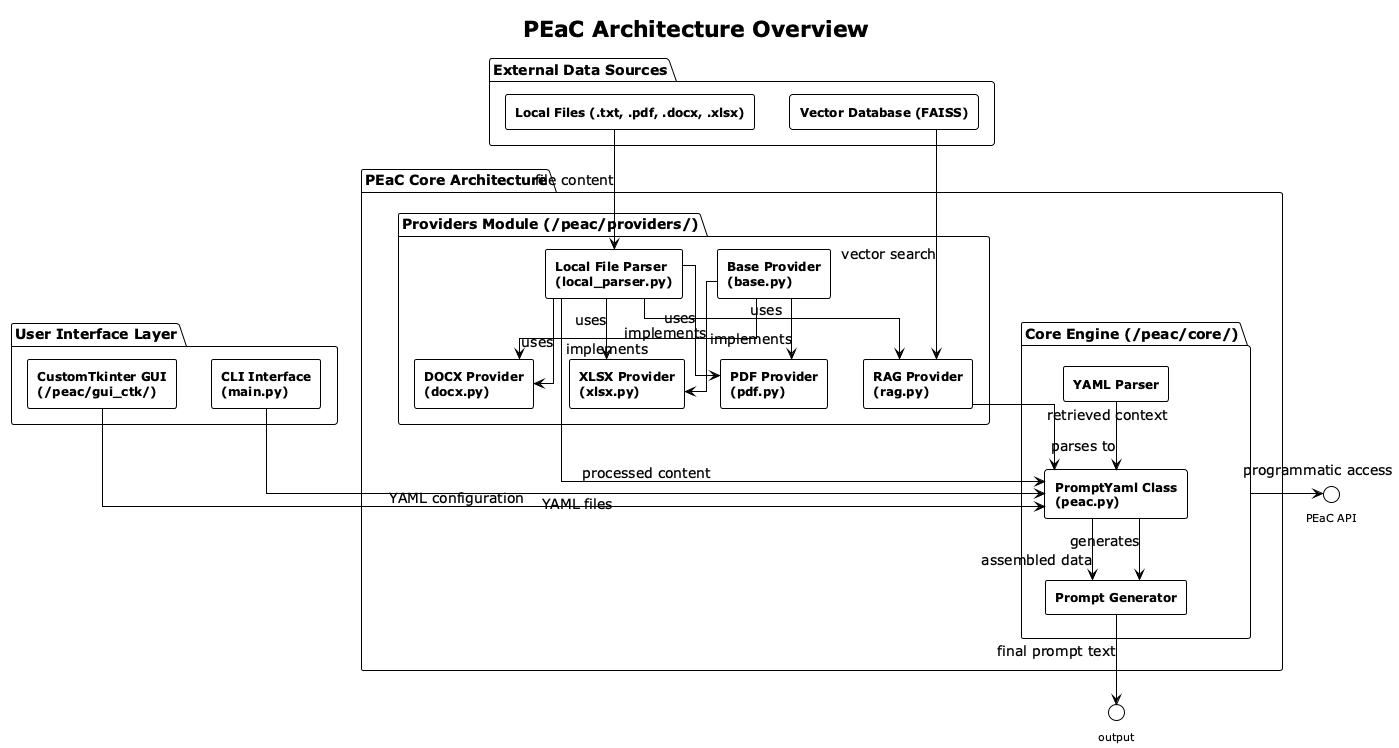
\includegraphics[width=0.8\linewidth]{figs/modules.png}
    \caption{PEaC architecture overview. The architecture consists of three main components: providers, the RAG module, and the interactive GUI. Providers are modules that allow the integration of external data sources into the generated final prompt. The Local Provider handles file system integration with filtering and recursive search capabilities. The Web Provider manages HTTP requests and content extraction with XPath support. The RAG Provider implements vector search and retrieval with configurable parameters. The RAG Module encompasses vector store management, embedding processing, and retrieval engine functionality. The Interactive GUI provides a user-friendly CustomTkinter-based interface for creating and managing YAML configurations, while the CLI offers terminal-based automation support. The Core Engine integrates YAML parsing, template processing, and prompt generation to produce structured prompts compatible with various language models including ChatGPT and Claude.}
    \label{fig:modules}
\end{figure}

% Alternative detailed description for methods section:
% The PEaC framework architecture (Figure~\ref{fig:modules}) implements a modular design consisting of three primary architectural layers: 
% (i) External Data Sources layer supporting local files (.txt, .pdf, .docx, .xlsx), web resources via HTTP/HTTPS, and vector databases using FAISS indexing; 
% (ii) PEaC Core Architecture encompassing specialized providers (Local, Web, RAG), a dedicated RAG module for vector-based retrieval, and the core engine for YAML parsing and prompt generation; 
% (iii) User Interface Layer providing both graphical (CustomTkinter-based GUI) and command-line interfaces for workflow automation.
% Data flows bidirectionally through the system, with providers abstracting the complexity of different data sources while maintaining consistent interfaces for the core processing engine.
% The RAG module implements semantic search capabilities through vector embeddings, enabling context-aware prompt enhancement.
% The resulting architecture supports reproducible prompt engineering workflows while maintaining modularity for extensibility and integration with existing LLM pipelines.